\documentclass[a4paper,12pt]{report}
%%%%%%%%%%%%%%%%%%%%%%%%%%%%%%%%%%%%%%%%%%%%%%%%%%%%%%%%%%%%%%%%%%%%%%%%%%%%%%%%%%%%%%%%%%%%%%%%%%%%%%%%%%%%%%%%%%%%%%%%%%%%%%%%%%%%%%%%%%%%%%%%%%%%%%%%%%%%%%%%%%%%%%%%%%%%%%%%%%%%%%%%%%%%%%%%%%%%%%%%%%%%%%%%%%%%%%%%%%%%%%%%%%%%%%%%%%%%%%%%%%%%%%%%%%%%
\usepackage{eurosym}
\usepackage{vmargin}
\usepackage{amsmath}
\usepackage{graphics}
\usepackage{epsfig}
\usepackage{subfigure}
\usepackage{fancyhdr}
%\usepackage{listings}
\usepackage{framed}
\usepackage{graphicx}

\setcounter{MaxMatrixCols}{10}
%TCIDATA{OutputFilter=LATEX.DLL}
%TCIDATA{Version=5.00.0.2570}
%TCIDATA{<META NAME="SaveForMode" CONTENT="1">}
%TCIDATA{LastRevised=Wednesday, February 23, 2011 13:24:34}
%TCIDATA{<META NAME="GraphicsSave" CONTENT="32">}
%TCIDATA{Language=American English}

\pagestyle{fancy}
\setmarginsrb{20mm}{0mm}{20mm}{25mm}{12mm}{11mm}{0mm}{11mm}
\lhead{MA4128} \rhead{Mr. Kevin O'Brien}
\chead{Advanced Data Modelling}
%\input{tcilatex}


% http://www.norusis.com/pdf/SPC_v13.pdf
\begin{document}


%SESSION 1: Hierarchical Clustering
% Hierarchical clustering - dendrograms
% Divisive vs. agglomerative methods
% Different linkage methods

%SESSION 2: K-means Clustering

\tableofcontents

\chapter{Linkage}
\section{Linkage Methods for Cluster Analysis}
Having selected how we will measure distance, we must now choose the clustering algorithm, i.e. the rules that govern between which points distances are measured to determine cluster membership. There are many methods available, the criteria used differ and hence
different classifications may be obtained for the same data. This is important since it tells us that, although cluster analysis may provide an objective method for the clustering of cases, there can be subjectivity in the choice of method. 

The linkage distances are calculated by SPSS. The goal of the clustering algorithm is to join objects together into successively larger clusters, using some measure of similarity or distance. SPSS provides seven clustering algorithms, the most commonly used one being  \textbf{\textit{Ward's method}}.


\section{Summary of Linkage methods}
\begin{itemize}
	\item  Single linkage (minimum distance)
	\item  Complete linkage (maximum distance)
	\item  Average linkage
\end{itemize}

%http://www.rdg.ac.uk/~aes02mm/supermarket.sav

\subsubsection{Ward's method}
\begin{itemize}
	\item  Compute sum of squared distances within clusters
	\item  Aggregate clusters with the minimum increase in the
	overall sum of squares
\end{itemize}
\subsubsection{Centroid method}
The distance between two clusters is defined as the
difference between the centroids (cluster averages)


% http://www.norusis.com/pdf/SPC_v13.pdf
\subsection{Centroid method}
Here the centroid (mean value for each variable) of each cluster is calculated and the
distance between centroids is used. Clusters whose centroids are closest together are
merged. This method is also fairly robust.

\subsection{Nearest neighbour method} 
\begin{itemize}
	\item A commonly used approach in hierarchical clustering is \textbf{\textit{Ward’s linkage method}}.
	This approach does not combine the two most similar objects successively. Instead,
	those objects whose merger increases the overall within-cluster variance to the
	smallest possible degree, are combined. If you expect somewhat equally sized
	clusters and the data set does not include outliers, you should always use Ward’s
	method.
	
	We will use the Ward's linkage method for laboratory exercises.
	
	\item Other most popular
	agglomerative clustering procedures include the following:
	\begin{description}
		\item[Single linkage (nearest neighbor)]: The distance between two clusters corresponds
		to the shortest distance between any two members in the two clusters.
		\begin{figure}[h!]
			\begin{center}
				% Requires \usepackage{graphicx}
				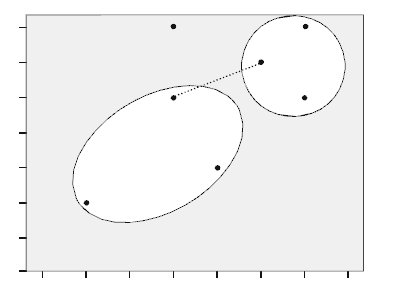
\includegraphics[scale=0.4]{images/Link1.jpg}\\
			\end{center}
		\end{figure}
		\item[Complete linkage (furthest neighbor)]: The oppositional approach to single
		linkage assumes that the distance between two clusters is based on the longest
		distance between any two members in the two clusters.
		\begin{figure}[h!]
			\begin{center}
				% Requires \usepackage{graphicx}
				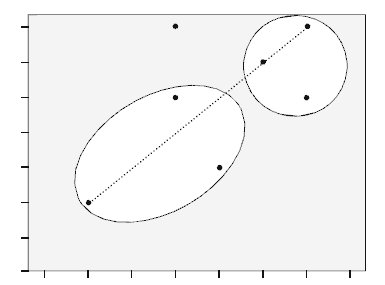
\includegraphics[scale=0.4]{images/Link2.jpg}\\
			\end{center}
		\end{figure}
		\item[Average linkage] : The distance between two clusters is defined as the average
		distance between all pairs of the two clusters’ members.
		\begin{figure}[h!]
			\begin{center}
				% Requires \usepackage{graphicx}
				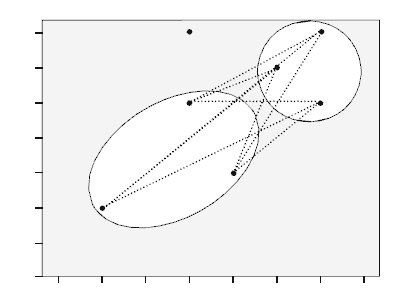
\includegraphics[scale=0.4]{images/Link3.jpg}\\
			\end{center}
		\end{figure}
		\newpage
		\item[Centroid] : In this approach, the geometric center (centroid) of each cluster is
		computed first. The distance between the two clusters equals the distance between
		the two centroids.
		\begin{figure}[h!]
			\begin{center}
				% Requires \usepackage{graphicx}
				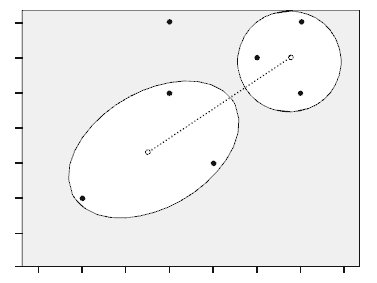
\includegraphics[scale=0.4]{images/Link4.jpg}\\
			\end{center}
		\end{figure}
	\end{description}
	Each of these linkage algorithms can yield totally different results when used on the same data set, as each has its specific properties. As the single linkage algorithm is based on minimum distances, it tends to form one large cluster with the other clusters containing only one or few objects each. We can make use of this \textbf{\textit{chaining effect}} to detect outliers, as these will be merged with the remaining objects – usually at very large distances – in the last steps of the analysis. Generally, single linkage is considered the most versatile algorithm.
	
	Conversely, the complete linkage method is strongly affected by outliers, as it is based on maximum distances. Clusters produced by this method are likely to be rather compact and tightly clustered. The average linkage and centroid algorithms tend to produce clusters with rather low within-cluster variance and similar sizes.
	However, both procedures are affected by outliers, though not as much as complete linkage.
\end{itemize}

\subsection{Nearest neighbour method} 
(Also known as the single linkage method).\\
In this method the distance between two clusters is defined to be the distance between
the two closest members, or neighbours. This method is relatively simple but is often
criticised because it doesn’t take account of cluster structure and can result in a problem
called chaining whereby clusters end up being long and straggly. However, it is better
than the other methods when the natural clusters are not spherical or elliptical in shape.

\subsection{Furthest neighbour method}
\textit{(Also known as the complete linkage method)}.\\
In this case the distance between two clusters is defined to be the maximum distance
between members  i.e. the distance between the two subjects that are furthest apart.
This method tends to produce compact clusters of similar size but, as for the nearest
neighbour method, does not take account of cluster structure. It is also quite sensitive
to outliers.


\subsection{Average (between groups) linkage method }
\textit{(sometimes referred to as Unweighted Pair Group Method with Arithmetic Mean (UPGMA)).}\\
The distance between two clusters is calculated as the average distance between all pairs
of subjects in the two clusters. This is considered to be a fairly robust method.


\subsection{Ward’s method}
In this method all possible pairs of clusters are combined and the sum of the squared
distances within each cluster is calculated. This is then summed over all clusters. The
combination that gives the lowest sum of squares is chosen. This method tends to
produce clusters of approximately equal size, which is not always desirable. It is also
quite sensitive to outliers. Despite this, it is one of the most popular methods, along
with the average linkage method.

%\subsection{Ward's Method}
%This method is distinct from other methods because it uses an \textbf{\textit{analysis of variance}} approach to evaluate the distances between clusters. In general, this method is very efficient.
%
%Cluster membership is assessed by calculating the total sum of squared deviations from the mean of a cluster. The criterion for fusion is that it should produce the smallest possible increase
%in the error sum of squares.
%
%
%
%\subsection{Ward's Linkage}
%
%Ward's linkage is a method for hierarchical cluster analysis . The idea has much in common with analysis of variance (ANOVA). The linkage function specifying the distance between two clusters is computed as the increase in the "error sum of squares" (ESS) after fusing two clusters into a single cluster. Ward's Method seeks to choose the successive clustering steps so as to minimize the increase in ESS at each step.


\subsection{Ward’s Linkage method (IMPORTANT)}
In this method all possible pairs of clusters are combined and the sum of the squared
distances within each cluster is calculated. This is then summed over all clusters. The
combination that gives the lowest sum of squares is chosen. This method tends to
produce clusters of approximately equal size, which is not always desirable. It is also
quite sensitive to outliers. Despite this, it is one of the most popular methods, along
with the average linkage method.

%\subsection{Ward's Method}
%This method is distinct from other methods because it uses an \textbf{\textit{analysis of variance}} approach to evaluate the distances between clusters. In general, this method is very efficient.
%
%Cluster membership is assessed by calculating the total sum of squared deviations from the mean of a cluster. The criterion for fusion is that it should produce the smallest possible increase
%in the error sum of squares.
%
%
%
%\subsection{Ward's Linkage}
%
%Ward's linkage is a method for hierarchical cluster analysis . The idea has much in common with analysis of variance (ANOVA). The linkage function specifying the distance between two clusters is computed as the increase in the "error sum of squares" (ESS) after fusing two clusters into a single cluster. Ward's Method seeks to choose the successive clustering steps so as to minimize the increase in ESS at each step.


%
%\subsection{Applications of Cluster Analysis}
%
%In medicine, the clustering of symptoms and diseases leads to taxonomies of illnesses. In the field of business, clusters of consumer segments are often sought for successful marketing strategies. Biologists have to organize the different species of animals before a meaningful description of the differences between animals is possible.

%\subsection{Cluster Analysis as a Statistical Tool}





%========================================================== %
Amalgamation or Linkage Rules
At the first step, when each object represents its own cluster, the distances between those objects are defined by the chosen distance measure. However, once several objects have been linked together, how do we determine the distances between those new clusters? In other words, we need a linkage or amalgamation rule to determine when two clusters are sufficiently similar to be linked together. There are various possibilities: for example, we could link two clusters together when any two objects in the two clusters are closer together than the respective linkage distance. Put another way, we use the "nearest neighbors" across clusters to determine the distances between clusters; this method is called single linkage. This rule produces "stringy" types of clusters, that is, clusters "chained together" by only single objects that happen to be close together. Alternatively, we may use the neighbors across clusters that are furthest away from each other; this method is called complete linkage. There are numerous other linkage rules such as these that have been proposed.
%=============================================================== %
Single linkage (nearest neighbor). As described above, in this method the distance between two clusters is determined by the distance of the two closest objects (nearest neighbors) in the different clusters. This rule will, in a sense, string objects together to form clusters, and the resulting clusters tend to represent long "chains."
Complete linkage (furthest neighbor). In this method, the distances between clusters are determined by the greatest distance between any two objects in the different clusters (i.e., by the "furthest neighbors"). This method usually performs quite well in cases when the objects actually form naturally distinct "clumps." If the clusters tend to be somehow elongated or of a "chain" type nature, then this method is inappropriate.
%=============================================================== %
Unweighted pair-group average. In this method, the distance between two clusters is calculated as the average distance between all pairs of objects in the two different clusters. This method is also very efficient when the objects form natural distinct "clumps," however, it performs equally well with elongated, "chain" type clusters. Note that in their book, Sneath and Sokal (1973) introduced the abbreviation UPGMA to refer to this method as unweighted pair-group method using arithmetic averages.
%================================================================ %
Weighted pair-group average. This method is identical to the unweighted pair-group average method, except that in the computations, the size of the respective clusters (i.e., the number of objects contained in them) is used as a weight. Thus, this method (rather than the previous method) should be used when the cluster sizes are suspected to be greatly uneven. Note that in their book, Sneath and Sokal (1973) introduced the abbreviation WPGMA to refer to this method as weighted pair-group method using arithmetic averages.
Unweighted pair-group centroid. The centroid of a cluster is the average point in the multidimensional space defined by the dimensions. In a sense, it is the center of gravity for the respective cluster. In this method, the distance between two clusters is determined as the difference between centroids. Sneath and Sokal (1973) use the abbreviation UPGMC to refer to this method as unweighted pair-group method using the centroid average.
%=============================================================== %
Weighted pair-group centroid (median). This method is identical to the previous one, except that weighting is introduced into the computations to take into consideration differences in cluster sizes (i.e., the number of objects contained in them). Thus, when there are (or we suspect there to be) considerable differences in cluster sizes, this method is preferable to the previous one. Sneath and Sokal (1973) use the abbreviation WPGMC to refer to this method as weighted pair-group method using the centroid average.
%=============================================================== %
Ward's method. This method is distinct from all other methods because it uses an analysis of variance approach to evaluate the distances between clusters. In short, this method attempts to minimize the Sum of Squares (SS) of any two (hypothetical) clusters that can be formed at each step. Refer to Ward (1963) for details concerning this method. In general, this method is regarded as very efficient, however, it tends to create clusters of small size.
%=============================================================== %



\end{document}